%======================================================================
\section{自适应拓扑路由}
\label{sec:topology}
%======================================================================

这项工作的一个关键见解是，没有任何单一的通信拓扑能够在所有问题上占据主导地位。我们将拓扑形式化为一个设计变量，并引入了自适应路由。

\subsection{通信拓扑}

我们将五种通信拓扑定义为加权邻接矩阵 $W \in \mathbb{R}^{n \times n}$：

\begin{itemize}
    \item \textbf{并行 (Parallel)} ($W = \mathbf{0}$)：所有智能体独立推理，智能体之间没有通信。这是标准的自洽性（self-consistency）设置。
    \item \textbf{顺序 (Sequential)} ($W$ = 路径图)：智能体 $i$ 观察智能体 $1, \ldots, i{-}1$ 的输出。信息单向流动，模仿智能体链架构。
    \item \textbf{星形 (Star)} ($W$ = 星形图)：一个中心节点智能体聚合所有叶节点智能体的输出，并生成综合结果。叶节点智能体独立推理。
    \item \textbf{辩论 (Debate)} ($W$ = 完全图，多轮)：所有智能体都观察所有其他智能体在上一轮中的结论。重复 3 轮，模拟多智能体辩论。
    \item \textbf{分层 (Hierarchical)} ($W$ = 两级树)：智能体被分成多个子组，首先进行内部协商，然后共享子组结论以进行跨组综合。
\end{itemize}

拓扑结构 $W$ 既影响信号计算（EV 和一致性信号依赖于邻居集 $\mathcal{N}_i$），也影响智能体行为（在顺序、星形、辩论和分层模式下的上下文感知生成）。

\subsection{单拓扑参数优化}

对于每种拓扑 $T \in \{\text{并行, 顺序, 星形, 辩论, 分层}\}$，我们通过基于特定拓扑信号的差分进化算法独立优化 $\theta^*_T$：
\begin{equation}
    \theta^*_T = \arg\max_{\theta \in \Theta} \; \text{Accuracy}_T(\theta) + \lambda \cdot \text{IC}_T(\theta)
\end{equation}

这产生了五种专门的共识配置。优化后的参数揭 示了特定拓扑的结构特性（图~\ref{fig:theta}）：星形和辩论拓扑为 EV 学习到了接近于零的权重（$w_{\text{EV}} \approx 0.01$），抑制了阿谀奉承风险最高的跨智能体共识信号。分层和顺序拓扑则学习到了较高的共识压力（$\lambda_c > 4.5$），强制在其链式/树状结构内达成一致。

\begin{figure}[t]
\centering
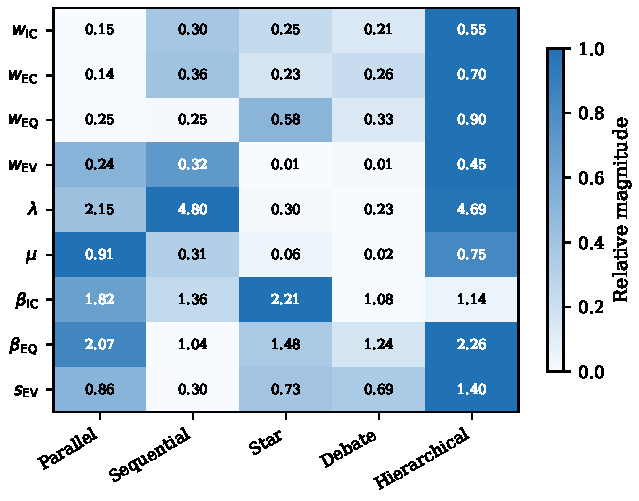
\includegraphics[width=0.72\columnwidth]{figures/fig_theta_heatmap.pdf}
\caption{逐拓扑优化参数 $\theta^*_T$（问答领域验证）。星型与辩论拓扑学到接近零的 EV 权重——涌现出的反谄媚配置；层级与顺序拓扑学到高共识压力 $\lambda_c$。}
\label{fig:theta}
\end{figure}

\subsection{神经拓扑路由器}
\label{sec:router}

为了为每个问题选择最佳拓扑，我们使用从 AEIC 结构化输出中提取的特征训练了一个神经路由器。

\paragraph{特征设计。} 对于每个候选拓扑 $T$，我们构建了一个 42 维的特征向量，包含每个智能体的质量信号（5 个智能体的 IC、EC、EQ、EV 和一致性）、汇总统计量（均值、标准差、范围）、\emph{投票特征}（多数比例、从 AEIC 结论中提取的“是/否”分布）以及跨信号交互特征（例如，$\text{IC}_i \times (1{-}\text{agreement}_i)$）。另外还有一个 7 维的问题级特征向量，用于捕捉文本特征和跨拓扑的信号方差。正如第~\ref{sec:exp} 节所示，得益于 AEIC 结构化结论提取的支持，投票特征是路由器准确性的主要驱动因素（引入后提升 $+2.1$ 个百分点），而几个质量信号组的贡献微乎其微甚至为负。

\paragraph{路由器架构。} 一个\emph{共享拓扑编码器}（包含 LayerNorm 和 GELU 的两层网络，维度从 42 映射到 96）处理每个拓扑的特征。一个\emph{上下文投影层}总结其他四种拓扑的嵌入表示（48 维）。三个\emph{针对特定数据集的评分头}将拼接后的表示（192 维）映射为标量分数，从而实现针对特定数据集的路由选择。

\paragraph{训练。} 我们使用具有自适应边距的焦点排序损失（focal ranking loss）：
\begin{equation}
    \mathcal{L} = \sum_{(c, w)} \left(\frac{v}{m}\right)^\gamma \cdot v, \quad v = \max(0, \; m - (s_c - s_w))
\end{equation}
其中 $(c, w)$ 是（正确，错误）拓扑对，$m$ 是适应难度的边距，$\gamma = 3$ 提供了焦点加权。训练使用 AdamW 优化器，带余弦退火策略，训练 300 个 epoch，并使用 5 折分层交叉验证。

\paragraph{Top-1 选择。} 路由器选择每个问题得分最高的拓扑作为共识拓扑。凭借针对特定数据集的专门评分头，该方法在 5 个随机种子上实现了 87.6\% $\pm$ 0.3\% 的准确率（5 折交叉验证），而最佳固定拓扑（星形）的准确率为 83.1\%。训练用的正确性标签使用多数投票结果，而不是 Stackelberg 加权决策，以避免受优化的 $\theta^*$ 参数污染。